%\begin{figure}[h]
%	\includegraphics[width=\columnwidth]{images/cat.jpg}
%	\caption{A very cute cat.}
%	\label{figure:cat}
%	\centering
%\end{figure}

%See \autoref{figure:cat}, such a cute cat!

\begin{quote}
"Debugging is twice as hard as writing the code in the first place. Therefore, if you write the code as cleverly as possible, you are, by definition, not smart enough to debug it." \\
\hspace*{\fill} — Brian Kernighan 
\end{quote}

The task for Milestone 2 was to implement a system for managing virtual memory. This can be broken down into the following modules


\subsubsection*{A Model of the Page Table}

To map a given physical address to a virtual address on ARMv8, one must install an entry into the corresponding L3 page table. Due to the capability system present in Barrelfish, the user process wishing to perform this mapping must posses a capability to that particular page table. This means that the memory server must keep around an in-memory model of the actual page table. 

There are a number of data structures one could use to encode this information, with the requirements being to maintain fast access and minimal memory footprint. There were two such structures that immediately stuck out:


\begin{itemize}
\item A \textbf{hash-table} would have a minimal memory footprint and provide very fast access. Deciding what to hash on here presents some difficulties, though. A simple approach would be to hash the index bits of the virtual address, and store the L3 page table along with a linked list of its parent page tables at that location. One could always find a necessary L2 page table by simply looking for the 0'th index L3 with those L2 index bits, and so on. This approach is fast! But still involves a number of layers of indirection. If there was a simple way to construct a \textit{flat} hash table to keep track of all of the page table capabilities we needed, that would be an ideal approach.

\item A \textbf{tree }in which each node contains an array of pointers to its children provides both a minimal memory footprint and constant-time lookup. There is a performance hit incurred from introducing between 3 and 6 levels of indirection (depending on whether the array of children is integral or allocated elsewhere), but the structure is simple and easy to manage. On top of the simplicity, the code for this structure models well the mental image of the tree of tables, making reasoning about it far easier. This is the approach we elected to follow through with. See \autoref{figure:page_table}.
\end{itemize}

\begin{figure}[h]
	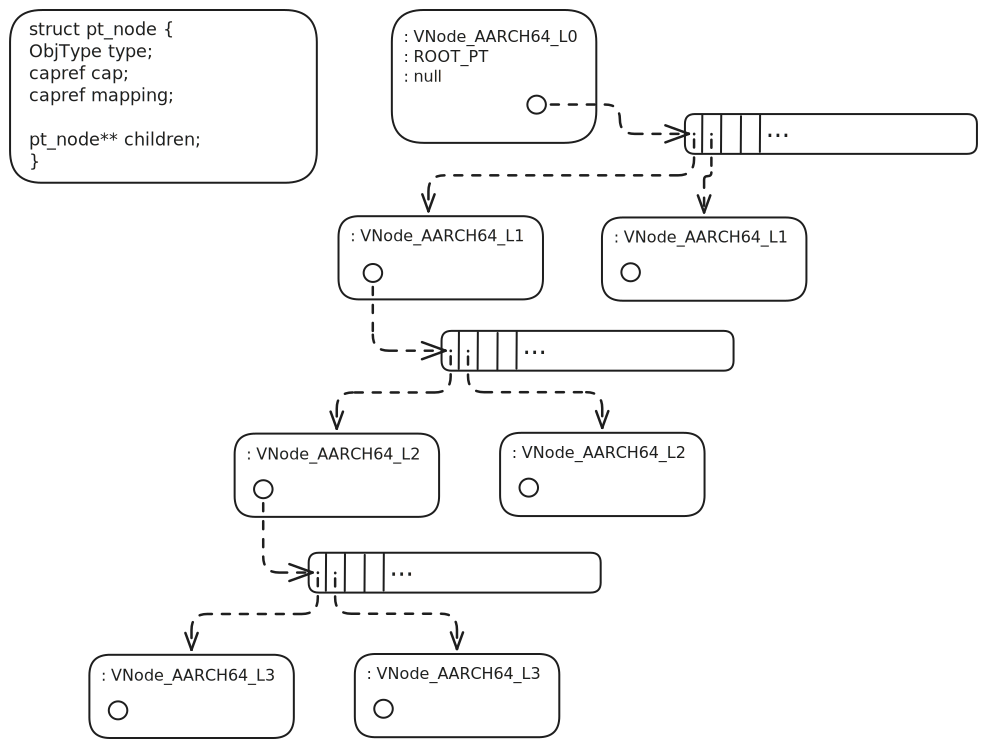
\includegraphics[width=\columnwidth]{report/images/page_table.png}
	\caption{Our representation of the page table}
	\label{figure:page_table}
	\centering
\end{figure}

\subsubsection*{Free, Allocated, and Mapped Memory}

In order to manage and distribute virtual address ranges, we must have some structure to keep track of which regions of the virtual address space are free to be given out, and which are reserved. Additionally, since we require the ability to lazily back these regions with physical memory, we differentiate between allocated (reserved but not backed) and mapped (backed with physical memory). The operations that the virtual memory system must provide are as follows,
\begin{enumerate}
    \item Find a free region of memory and allocate it.
    \item Find a free region of memory and map it
    \item Allocate a specific region of memory
    \item Map a specific region of memory
\end{enumerate}

Some of the operations turn out to be a lot more important than others in Barrelfish. Our key concern in designing this part of our virtual memory system was speed of backing virtual memory in the case of a page fault. Our design makes limited use of allocation and freeing of virtual memory regions, which is explained in the later \autoref{heap} discussing our implementation of the \textbf{heap}. This means that the most frequent virtual memory operation that occurs is a traversal of our virtual memory region structure in order to determine whether an address that triggered a page fault should be mapped (is allocated) or should propagate the page fault as an error (is free).

We prioritize the speed of finding allocated but unmapped regions, and so an AVL tree storing ranges seemed like the obvious approach. By using a comparison function that checked to see if the provided range was a subset of any existing range in the tree, we could keep things balanced nicely. However, due to time constraints and messy development around this milestone, the initial approach we decided on was to keep a linked list of free and allocated regions to fetch from. A mapping operation, then, would remove a node from this list to be stored in an AVL tree. We failed to realize that this is an incredibly expensive operation to be performing for every page fault, and that optimizing the time it took to find a free region would make little difference to the performance of our allocator. See \autoref{figure:vmf_list} for a diagram of our region list.


\begin{figure*}[h] 
	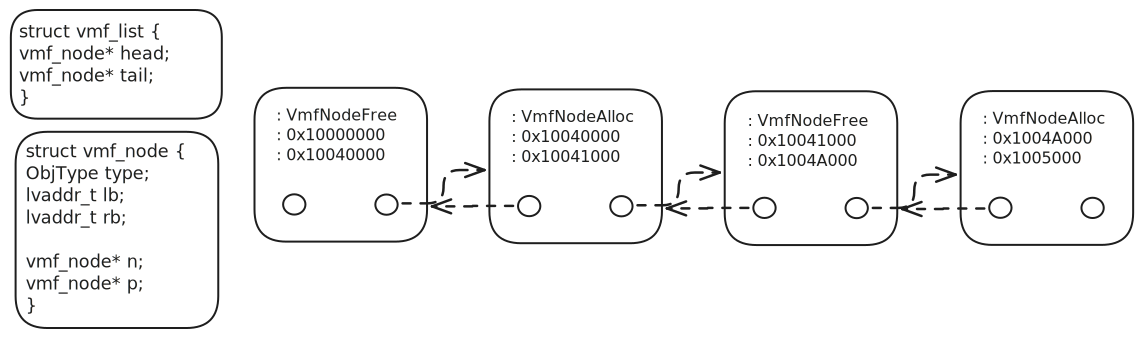
\includegraphics[width=\textwidth]{report/images/vmf_list.png}
	\caption{An initial approach: Keeping track of virtual memory regions}
	\label{figure:vmf_list}
	\centering
\end{figure*}

The page fault handler itself receives upcalls from the barrelfish kernel anytime a given virtual address not backed by any physical memory is touched. The goal of the handler is to verify whether this page fault resulted from a valid memory access, and if so, to perform the mapping operation.

\subsubsection*{The Heap} \label{heap}
Our heap functions by first reserving (allocating) a chunk of the virtual address space larger than the total available memory in the system. We then rely on the page fault handler and our other paging data structures to do the heavy lifting, lazily mapping chunks of this region when accesses occur. Using this approach, our actual \verb|morecore| consisted of very little code, and most of what was written serves setup and teardown.

\subsubsection*{Improvements} \label{improvements}

There are two lines of improvement we wanted to take with our allocation data structures. The first is simple, but halves the level of indirection involved in traversing our in-memory model of the page table. This is simply switching out the \verb|pt_node** children| member of the \verb|pt_node| struct for a \verb|ptr_node* children[]| flexible array member. This allows us to maintain the small memory footprint of L3 page table nodes, which have no children, while simplifying the allocation code. We didn't end up implementing this change due to time constraints.

The second, more involved change to make to our allocation data structures was to rip out our \verb|vmf_list| and simply use AVL trees to keep track of all memory regions. Our thought was that this would remove the $\mathcal{O}(n)$ bottleneck on all of our memory operations and streamline the paging code significantly by unifying our logic for manipulating these regions. However, this did not end up being the case. 


\begin{figure}[h] 
	\includegraphics[width=\columnwidth]{report/images/rpc_lmp(1).png}
	\caption{The free region tree}
	\label{figure:vmf_tree}
	\centering
\end{figure}

In testing, we found that using two separate AVL trees, one for free and allocated regions, the other storing mapped regions, was in fact slower in almost all cases. Allocation suffered a huge performance hit, as now instead of a simple linked list split, we had to rebalance an AVL tree. With the number of nodes we were working with in this memory allocator, this simply did not add up to a reasonable tradeoff.

The unexpected part of this is that mapping and unmapping remained largely unchanged. We can interpret from this that, even with the initial linked list implementation, the cost of AVL tree operations dominates. \autoref{figure:performance} illustrates the performance characteristics of using a linked list vs an AVL tree to implement our free and allocated regions tracking data structure.


\begin{figure}[h] 
	\includegraphics[width=\columnwidth]{report/images/AVL Tree V. Linked List Performance.png}
	\caption{Performance characteristics}
	\label{figure:performance}
	\centering
\end{figure}